% !TeX TXS-program:compile = txs:///pdflatex/[--shell-escape]



% #######################################
% ######### Параметры документа #########
% #######################################

% 14-й шрифт (стандарт для дипломных работ) %
\documentclass[a4paper,14pt]{extarticle}
% 12-й шрифт %
%\documentclass[12pt, a4paper]{article}

% Кодировки требуются только если компилятор не включает поддержку Unicode
% (поддержку по умолчанию имеют XeTeX, LuaLaTeX)
\usepackage[utf8x]{inputenc}
\usepackage[T1, T2A]{fontenc}
\usepackage[english,russian]{babel}

% Стилевой файл %
\usepackage[spisok,boldsect,eqwhole,figwhole,hyperref,hyperprint,greekit]{fn2style/fn2kursstyle}

% Междустрочный интервал 1.5 %
\usepackage{setspace}
\setstretch{1.5}

% Размер полей %
\usepackage[left=3cm,right=1cm, top=2cm,bottom=2cm]{geometry}

% Включение титульника PDF %
\usepackage{pdfpages}

% Меняем нумерацию страниц с красивой на снизу по центру %
\pagestyle{plain}

% multline внутри других оболочек %
\usepackage{mathtools}

% Центрированные таблицы фиксированной ширины %
\usepackage{tabularx} % also loads 'array' package
\newcolumntype{C}{>{\centering\arraybackslash}X} % centered version of 'X' columns

% 2-я страница оглавления начинается без отступа сверху %
\usepackage[titles]{tocloft}
% Т.е. используем tocloft, требуется явно указать что основные разделы заполняют простанство до станиц точками %
\renewcommand{\cftsecleader}{\cftdotfill{\cftdotsep}}

% Фикс для false-positive warning'ов из bibliography %
% (bibliography использует \sloppy чтобы несколько ослабить правила переноса, но \sloppy не трогает анализатор hbadness, который начинает давать false-positive предупреждения о "некрасивых" переносах строки) %
\usepackage{etoolbox}
\apptocmd{\sloppy}{\hbadness 10000\relax}{}{}

% Алгоритмы %
\usepackage{algorithm2e} % texlive-science
\RestyleAlgo{ruled}
\SetKwData{Assume}{Assumptions}

% Уменьшаем пробел вокруг ":" в формулах %
\DeclareMathSymbol{:}{\mathord}{operators}{"3A}

% Делаем verbatim меньше %
\usepackage{verbatim}

\newenvironment{smallverbatim}%
{\small\verbatim}%
{\endverbatim}

\newenvironment{tinyverbatim}%
{\footnotesize\verbatim}%
{\endverbatim}

% Путь к графике %
\graphicspath{{./style/}{./images/}}



% ######################################
% ######### Кастомные комманды #########
% ######################################

% d %
\newcommand*\diff{\mathop{}\!\mathrm{d}}
% 1/2 %
\newcommand{\half}{{1/2}}
% Div %
\renewcommand{\div}{\mathrm{div}}
% Grad %
\newcommand{\grad}{\mathrm{grad}}
% Const %
\newcommand{\const}{\mathrm{const}}
% E %
\newcommand{\E}{\mathbb{E}}
% D %
\newcommand{\D}{\mathbb{D}}
% D %
\newcommand{\K}{\mathbb{K}}
% = by def %
\newcommand\eqbydef{\mathrel{\overset{\makebox[0pt]{\mbox{\normalfont\tiny\sffamily def}}}{=}}}
% epsilon %
\renewcommand{\epsilon}{\varepsilon}
% Re %
\renewcommand{\Re}{\ensuremath{\,\textrm{Re}}}
% Im %
\renewcommand{\Re}{\ensuremath{\,\textrm{Im}}}
% Vector %
\renewcommand{\vec}{\bi}
% e %
\newcommand{\euler}{\mathrm{e}}
% dirac delta %
\newcommand{\diracdelta}{\delta}
% green function G %
\newcommand{\greenfunc}{\mathrm{G}}
% erf %
\newcommand{\erf}{\mathrm{erf}}
% Wide tilde %
\newcommand{\wt}{\widetilde}
% Wide tilde %
\newcommand{\forany}{\forall}

% Запятая в индексах
\newcommand{\idxcomma}{,\;}

% Shortcut для дифференцирования по 1 аргументу

\newcommand{\dpartial}[2]{\dfrac{\partial #1}{\partial #2}}

\newcommand{\dfull}[2]{\dfrac{\diff #1}{\diff #2}}

% Маленький верхний индекс %
\usepackage{relsize}
\newcommand{\smallalpha}{\mathsmaller{(} \alpha \mathsmaller{)}}
\newcommand{\smallbeta}{\mathsmaller{(} \beta \mathsmaller{)}}

% Осреднение по ансамблю %
\newcommand{\avg}[1]{\left\langle #1 \right\rangle}

% Временные комментарии %
\newcommand{\intextnote}[2]{\begin{center}{\color{#2}\textbf{
	\rule{\textwidth}{2.0pt}
	\\ #1 \\
	\rule{\textwidth}{2.0pt}
}}\end{center}}

\newcommand{\COMMENT}[1]{\intextnote{#1}{red}}
\newcommand{\NOTE}[1]{\intextnote{#1}{blue}}

\newcommand{\appwidth}{6.45cm}

% {gather} для использования в тексте - не добавляет вертикальных пробелов %
\newenvironment{inlinegather*}{\par\centering$\displaystyle\begin{aligned}}{\end{aligned}$\par}


% ~~~~~~~~~~~~~~~~~~~~~~~~~~~~~~~~~~~~~~~~~~~~~~~~~~~~~~~~~~~~~~~~~~~~~~~~~~~~~~~~~~~~~~~~~~~~~~~~~~~~~~

\begin{document}

\title{"Методы численного решения задача линейной алгебры"}
\group{ФН2\,--\,31М}
\author{Д.\,И.~Богданов}
\supervisor{А.\,С.~Родин}
\date{2024}
\maketitle

% ==================
% --- Оглавление ---
% ==================

\newpage
\tableofcontents
\newpage


\section{Постановка задачи}


Нужно сформировать матрицу размером $10 \times 10$ по следующему принципу. В качестве базовой матрицы $А$, берется известная матрица, которая получается после дискретизации одномерного оператора Лапласа методом конечных разностей или методом конечных элементов. На равномерной сетке:
\[
A_0 = \left\lbrace a_{ij} \right\rbrace_{i, j = \overline{1, n}}
\]
где
\[
a_{ij} = \begin{cases}
2, \quad &i = j, \\
-1, \quad &|i-j| = 1, \\
0, \quad &\text{else}. \\
\end{cases}
\]
Для данной матрицы известны аналитические формулы для собственных значений ($n = 10$)
\[
\lambda_j^0 =2 (1 - \cos \dfrac{\pi j}{n + 1}),
\quad j = \overline{1, n}.
\]
и компонент собственных векторов (вектора имеют $2$-норму равную $1$):
\[
z_j^0 (k) = \sqrt{\dfrac{2}{n+1}} \sin \dfrac{\pi j k}{n+1},
\quad k = \overline{1, n}.
\]
Итоговая матрица получается по формулам:
\begin{gather*}
A = A_0 + \delta A, \\
\delta A_{ij} = \begin{cases}
\dfrac{c}{i + 1}, \quad &i \neq j, \\
0, \quad &i = j,
\end{cases} \\
c = \dfrac{N_{var}}{N_{var} + 1} \epsilon.
\end{gather*}
где $N_{var}$ --- номер варианта (совпадает с номером студента в списке в журнале
группы), $\epsilon$ - параметр, значение которого задается далее.

\subsection{Задание 1}

Взять матрицу $А$ для значения $\epsilon = 0.1$, убрать последний столбец и сформировать из первых $9$ столбцов матрицу $\hat{A}$ размера $10 \times 9$. Решить линейную задачу наименьших квадратов для вектора невязки
\[
r = \hat{A} x - b,
\]
где вектор $b$ размерности $10 \times 1$ нужно получить по следующему алгоритму: выбрать вектор $x_0$, размерности $9 \times 1$ и для него вычислить $b = \hat{А} х_0$.

Для решения поставленной задачи использовать QR разложение: для вариантов с четным номером использовать соответствующий алгоритм, основанный на методе вращений Гивенса, для вариантов с нечетным номером - алгоритм, основанный на методе отражений Хаусхолдера.

После получения решения сделать оценку величины $|| x - x_0 ||_2 / ||x_0||_2$.

\subsection{Задание 2}

Для матрицы $А$ найти все ее собственные значения ($\lambda_j, j = \overline{1, 10}$) и собственные вектора ($z_j, j = \overline{1, 10}$, с $2$-нормой равной $1$) с помощью неявного QR-алгоритма со сдвигом (с предварительным приведением матрицы к форме Хессенберга) для трех вариантов: $\epsilon = 10^{-1}, 10^{-3}, 10^{-6}$.

По итогам расчетов нужно сделать сводную таблицу, в которой указать следующие величины: $\lambda_j - \lambda_j^0$ и $||z_j - z_j^0||_2$ для $j = \overline{1, 10}$.

\section{Решение линейной задачи наименьших квадратов в с помощью QR-разложения методом отражений Хаусхолдера}

В рамках данной задачи реализованы следующие алгоритмы:
\begin{itemize}
\item Отражение Хаусхолдера;

\item Обычное QR-разложение;

\item QR-разложение для метода LLS;

\item Обратный ход метода Гаусса;

\item Linear Least Squares с помощью QR-разложения.
\end{itemize}

Расчетная реализация всех алгоритмов выполнена на языке \texttt{C++} с использованием библиотеки \texttt{Eigen} для базовых матричных операций. Для отладки программы и проверки корректности результатов реализован вспомогательный скрипт на \texttt{Wolfram Mathematica}, использующий встроенные методы для получения необходимых разложений. При указании асимптотической сложности алгоритмов далее будет подразумеваться $m \sim n$.

\subsection{QR-разложение и его эффективная реализация}

Алгоритм QR-разложения имеет следующий вид:

\begin{algorithm}[H] % 'H' makes environment non-float
\caption{QR Factorization (naive)}
\vspace{4pt}
\KwData{$n \leq m$}
\KwIn{$A_{m \times n}$}
\KwOut{$Q_{m \times n}$, $R_{n \times n}$}
$\tilde{Q} \gets I_{m \times m}$\;
$\tilde{R} \gets A_{m \times n}$\;
\For{$i \gets 1$, $i \leq \min \lbrace m-1, n \rbrace$, $i \gets i + 1$} {
	$k \gets m - i$\;
	$u_i \gets \mathrm{HouseholderReflection}(\tilde{R}[i:m, i])_{k \times 1}$\;
	$\tilde{P}_i \gets I_{k \times k} - 2 u_i u_i^T$\;
	$P_i \gets I_{m \times m}$\;
	$P_i[i:m, i:m] \gets \tilde{P}_i$\;
	$\tilde{Q} \gets \tilde{Q} \cdot P_i$\;
	$\tilde{R} \gets P_i \cdot \tilde{R}$\;
}
$Q \gets \tilde{Q}[1:m, 1:n]$\;
$R \gets \tilde{R}[1:n, 1:n]$\;
\end{algorithm}
\vspace{8pt}

\noindent Записанный в явном виде алгоритм QR-разложения имеет сложность $O(n^4)$ в силу наличия матричного умножения, это решается если подставить матрицу $P_i$ явно и расписать матричные умножения как $2$ умножения матрицы на вектор. Приходим к алгоритму, эффективному для практической реализации:

\begin{algorithm}[H]
\caption{QR Factorization}
\vspace{4pt}
\KwData{$n \leq m$}
\KwIn{$A_{m \times n}$}
\KwOut{$Q_{m \times n}$, $R_{n \times n}$}
$\tilde{Q} \gets I_{m \times m}$\;
$\tilde{R} \gets A_{m \times n}$\;
\For{$i \gets 1$, $i \leq \min \lbrace m-1, n \rbrace$, $i \gets i + 1$} {
	$k \gets m - i$\;
	$u_i \gets \mathrm{HouseholderReflection}(\tilde{R}[i:m, i])_{k \times 1}$\;
	$\tilde{Q}[1:m, i:m] \gets \tilde{Q}[1:m, i:m] - 2 \tilde{Q}[1:m, i:m] \cdot u_i \cdot u_i^T$\;
	$\tilde{R}[i:m, i:n] \gets \tilde{R}[i:m, i:n] - 2 u_i \cdot (u_i^T \cdot \tilde{R}[i:m, i:n])$\;
}
$Q \gets \tilde{Q}[1:m, 1:n]$\;
$R \gets \tilde{R}[1:n, 1:n]$\;
\end{algorithm}
\vspace{8pt}

\noindent Полученный алгоритм имеет сложность $O(n^3)$. Далее, под QR-разложением будет подразумеваться именно эта реализация. $\mathrm{HouseholderReflect()}$ в данном случае является вспомогательной процедурой, имеющей сложность $O(n)$:

\vspace{8pt}
\begin{algorithm}[H]
\caption{Householder Reflection}
\vspace{4pt}
\KwIn{$x_{k \times 1}$}
\KwOut{$u_{k \times 1}$}
$u \gets x_{k \times 1}$\;
$u[1] \gets \mathrm{sign}(u[1]) ||u||_2$\;
$u \gets u / ||u||_2$\;
\end{algorithm}
\vspace{8pt}

\subsection{Алгоритм LLS и вспомогательные процедуры}

Алгоритм линейной задачи наименьших квадратов имеет следующий вид:

\vspace{8pt}
\begin{algorithm}[H]
\caption{LLS}
\vspace{4pt}
\KwData{$n \leq m$}
\KwIn{$A_{m \times n}$, $b_{m \times 1}$}
\KwOut{$x_{m \times 1}$}
$\lbrace Q, R \rbrace \gets \mathrm{QRFactorization}(A)$\;
$x \gets \mathrm{GaussianBackwardsElimination}(R, Q^T \cdot b)$\;
\end{algorithm}
\vspace{8pt}

\noindent тут $\mathrm{GaussianBackwardsElimination()}$ --- процедура обратного хода метода Гаусса, имеет следующую реализацию:

\begin{algorithm}[H]
\caption{Gaussian Backwards Elimination}
\vspace{4pt}
\KwData{$A$ is upper-triangular}
\KwIn{$R_{n \times n}$, $rhs_{n \times 1}$}
\KwOut{$x_{n \times 1}$}
$x \gets rhs_{n \times 1}$\;
\For{$i \gets n$, $i \geq 1$, $i \gets i - 1$} {
	\For{$j \gets i + 1$, $j \leq n$, $j \gets j + 1$} {
		$x[i] \gets x[i] - R[i, j] \cdot x[j]$\;
	}
	$x[i] \gets x[i] / R[i, i]$\;
}
\end{algorithm}
\vspace{8pt}

\subsection{Улучшение алгоритма LLS}

Алгоритм $\mathrm{LLS}$ можно улучшить если встроить вычисление правой части $Q^T b$ сразу в $\mathrm{QRFactorization}$. Получим следующую модификацию QR-разложения:

\begin{algorithm}[H]
\caption{QR Factorization for LLS}
\vspace{4pt}
\KwData{$n \leq m$}
\KwIn{$A_{m \times n}$, $b_{m \times 1}$}
\KwOut{$\beta_{n \times 1}, \; R_{n \times n}$}
$\tilde{\beta} \gets b_{m \times 1}$\;
$\tilde{R} \gets A_{m \times n}$\;
\For{$i \gets 1$, $i \leq \min \lbrace m-1, n \rbrace$, $i \gets i + 1$} {
	$k \gets m - i$\;
	$u_i \gets \mathrm{HouseholderReflection}(\tilde{R}[i:m, i])_{k \times 1}$\;
	$\gamma \gets -2 u_i^T \cdot \tilde{\beta}[i:m]$\;
	$\tilde{\beta}[i:m] \gets \tilde{\beta}[i:m] + \gamma \cdot u_i$
	$\tilde{R}[i:m, i:n] \gets \tilde{R}[i:m, i:n] - 2 u_i \cdot (u_i^T \cdot \tilde{R}[i:m, i:n])$\; 
}
$\beta \gets \tilde{\beta}[1:n]$\;
$R \gets \tilde{R}[1:n, 1:n]$\;
\end{algorithm}
\vspace{8pt}

\noindent Соответсвенно, разложение в $\mathrm{LLS}$ станет происходить не в $\lbrace Q, R \rbrace$, а сразу в матрицу и вектор правой части СЛАУ $\lbrace Q^T b, R \rbrace$.

\subsection{Результаты}

Произведено тестовое QR-разложение матрицы $\hat{A}$, проверена ортогональность матрицы $Q$ и приблизительное совпадение $QR \approx A$. Результаты сходятся с разложением с помощью встроенного метода \texttt{QRDecomposition[]} в пакете \texttt{Wolfram Mathematica}:

В качестве тестового вектора выбран $x_0: x_i = i^2$. Для него решена задача наименьших квадратов относительно невязки, получен вектор $x_{LLS}$ имеющий следующую норму ошибки:
\[
err_{LLS} \approx 3.99 \cdot 10^{-16}.
\]

Результаты LLS также сверены с помощью скрипта.

\section{Получение собственных значений матрицы с помощью QR-алгоритма со сдвигами}

В рамках данной задачи реализованы следующие алгоритмы:
\begin{itemize}
\item Приведение матрицы к Хессенберговой форма;

\item QR-алгоритм без сдвигов (для отладочных целей);

\item $O(N^2)$ QR-разложение для верхне-хессенберговых матриц с вычислением $RQ$;

\item QR-алгоритм со сдвигами и приведением изначальной матрицы к Хессенберговой форме;

\item Метод обратной итерации для определения СВ.
\end{itemize}

\subsection{QR-алгоритм}

\begin{algorithm}[H]
\caption{QR-algorithm (naive)}
\vspace{4pt}
\KwIn{$A_{n \times n}$}
\KwOut{$T_{n \times n}$}
$T \gets A_{n \times n}$\;
\For{$it \gets 0$, $it \leq \mathrm{limit}$, $it \gets it + 1$} {
	$\sigma \gets \sigma_i$\;
	$\lbrace Q, R \rbrace \gets \mathrm{QRFactorization}(A - \sigma I)$\;
	$T \gets R \cdot Q + \sigma I$\;
}
\end{algorithm}
\vspace{8pt}

Результатом работы алгоритма является матрица $T$ из разложения Шура $A = Q^* T Q$, элементы главной диагонали данной матрицы являются собственными значениями соответствующего оператора.

Заметим, что на данном этапе сложно сформулировать хороший критерий остановки, поэтому итерируемся фиксированное число раз или до тех пор пока разница между итерациями не станет достаточно малой. Вопрос определения $\sigma_i$ также пока что не конкретезируется, в случае $\sigma_i = 0$ получаем метод обычной QR-итерации без сдвига. И то и другое будет конкретизировано в следующем разделе при улучшении метода.

Данный алгоритм требует $O(n^4)$ операций т.к. QR-разложение обходится в $O(n^3)$, матричное умножение также требует $O(n^3)$ и ожидаемое число итераций до сходимости считаем пропорциональным размеру.

\subsection{Улучшение алгоритма с помощью приведения к Хессенберговой форме и редукции размерности}

Приведенный выше алгоритм QR-итерации можно улучшить, внесем следующий набор изменений в логику метода:

\begin{enumerate}
\item Приведем матрицу $A$ к верхне-хессенберговой форме с помощью отражений Хаусхолдера (Hessenberg Reduction), данная операция корректна т.к. не меняет собственные числа матрицы, приведение к верхне-хессенберговой форме требует $O(n^3)$ операций;

\item Реализуем модификацию $\mathrm{QRFactorization}()$ для верхне-хессенберговых матриц, сложность разложения упадет с $O(n^3)$ до $O(n^2)$;

\item Встроим получение матрицы $RQ$ в процедуру QR-разложения, это позволит избежать явного умножения матриц и снизит сложность получения $RQ$ до $O(n^2)$, таким образом вся QR-итерация снизится с $O(n^4)$ до $O(n^3)$;

\item Выберем сдвиг $\sigma_i = T_{nn}$, данный выбор сдвига обеспечивает стремление последней строки к соответствующей строке матрицы Шура, итерации производим до тех пор пока значение $|T_{n, n-1}|$ не станет меньше некоторого $\epsilon$, после чего $n$-е значение на диагонали считаем найденым и редуцируем задачу к работе с блоком $(n - 1) \times (n - 1)$. Получили конкретизацию сдвига и условия остановки.
\end{enumerate}

Соответсвенно, алгоритм QR-итерации придет к виду:

\vspace{8pt}
\begin{algorithm}[H]
\caption{QR-algorithm}
\vspace{4pt}
\KwIn{$A_{n \times n}$}
\KwOut{$T_{n \times n}$}
$it \gets 0$\;
$k \gets n$\;
$T \gets \mathrm{HessenbergReduction}(A)_{n \times n}$\;
\While{$k \geq 2$ $\&$ $it \leq \mathrm{limit}$} {
	$\sigma \gets T[k, k]$\;
	$RQ \gets \mathrm{QRFactorizationForHessenberg}(A - \sigma I)_{k \times k}$\;
	$T[1:k, 1:k] \gets RQ$\;
	\If{$|T[k, k-1]| < \epsilon$}{
		$k \gets k - 1$\;
	}
}
\end{algorithm}
\vspace{8pt}

\noindent Вспомогательная процедура $\mathrm{HessenbergReduction}()$ имеет алгоритм:

\vspace{8pt}
\begin{algorithm}[H]
\caption{Hessenberg reduction}
\vspace{4pt}
\KwIn{$A_{n \times n}$}
\KwOut{$H_{n \times n}$}
$H \gets A_{n \times n}$\;
\For{$i \gets 1$, $i \leq n - 2$, $i \gets i + 1$} {
	$k \gets m - i - 1$\;
	$u_i \gets \mathrm{HouseholderReflection}(R[i+1:n, i])_{k \times 1}$\;
	$H[i+1:n, i:n] \gets H[i+1:n, i:n] - 2 u_i \cdot (u_i^T \cdot H[i+1:n, i:n])$\;
	$H[1:n, i+1:n] \gets H[1:n, i+1:n] - 2 H[1:n, i+1:n] \cdot u_i \cdot u_i^T$\;
}
\end{algorithm}
\vspace{8pt}

\noindent Использование отражений Хаусхолдера для редукции к верхне-хессенберговой форме во многом аналогично их применению в QR-разложении, с той разницей, что вместо обнуления всех $s_i$ поддиагональных элементов происходит обнуление $s_i - 1$.

QR-разложение в силу Хессенберговой формы матрицы можем записать работающее для блоков ширины $2$, что снизит сложность до $O(n^2)$:

\vspace{8pt}
\begin{algorithm}[H]
\caption{QR Factorization for Hessenberg matrices}
\vspace{4pt}
\KwData{$A$ is an upper-hessenberg matrix}
\KwIn{$A_{n \times n}$}
\KwOut{$Q_{n \times n}$, $R_{n \times n}$, $RQ_{n \times n}$}
$Q \gets I_{n \times n}$\;
$R \gets A_{n \times n}$\;
$V \gets \mathrm{Zero}_{n \times n}$\;
\For{$i \gets 1$, $i \leq n - 1$, $i \gets i + 1$} {
	$k \gets m - i$\;
	$u_i \gets \mathrm{HouseholderReflection}(R[i:i+1, i])_{k \times 1}$\;
	$Q[1:n, i:i+1] \gets Q[1:n, i:i+1] - 2 Q[1:n, i:i+1] \cdot u_i \cdot u_i^T$\;
	$R[i:i+1, i:n] \gets R[i:i+1, i:n] - 2 u_i \cdot (u_i^T \cdot R[i:i+1, i:n])$\;
	$V[i:i+1, i] \gets u_i$\; 
}
$RQ \gets R$\;
\For{$i \gets 1$, $i \leq n - 1$, $i \gets i + 1$} {
	$v_i \gets V[i:i+1, i]$\;
	$RQ[1:m, i:i+1] \gets RQ[1:m, i:i+1] - 2 RQ[1:m, i:i+1] \cdot v_i \cdot v_i^T$\;
}
\end{algorithm}
\vspace{8pt}

\noindent Заметим, что непосредственно для QR-алгоритма матрицы $Q$, $R$ не нужны, их расчет реализован для общности и для отладочных целей.

\subsection{Обратная итерация}

Зная собственные значения из разложения Шура, собственные векторы можем получить с помощью метода обратной итерации:

\vspace{8pt}
\begin{algorithm}[H]
\caption{Inverse iteration}
\vspace{4pt}
\KwIn{$A_{n \times n}$, $\lambda_0$}
\KwOut{$\lambda$, $z_{n \times 1}$}
$i \gets 0$\;
$x \gets \mathrm{Ones}_{n \times 1} / n$ \tcc*{$||x||_2 = 1$}
\Repeat{$|\lambda_i - \lambda_{i-1}| < \epsilon$} {
	$i \gets i + 1$\;
	$x \gets \mathrm{GaussianElimination}(A - \lambda_0 I, x)$\;
	$x \gets x / ||x||_2$ \tcc*{$||x||_2 = 1$}
	$\lambda_i \gets x^T \cdot A \cdot x$\;
}
$\lambda \gets \lambda_i$\;
$z \gets x_{n \times 1}$\;
\end{algorithm}
\vspace{8pt}

\noindent В данном случае $\mathrm{GaussianElimination}()$ является вспомогательной процедурой для решения СЛАУ, выбор конкретно данного метода существенным не является. В программе реализован вариант с частичным выбором ведущего элемента и предобуславливателем Якоби.

\subsection{Результаты}

Получены собственные значения и векторы матрицы $A$, результаты сравнения с аналитическими результатами приведены ниже для $\epsilon = 10^{-1}, 10^{-3}, 10^{-6}$:
\begin{center}
\begin{tabular}{|c|c|c|c|c|}
\hline
 j & $|\lambda_j^0 - \lambda_j|$ & Итераций до редукции & $||z_j^0 - z_j||_2$ & Обратных итераций \\
\hline
   $1$ &                         $0.0383792$ &                     $5$ &                  $0.0615102$ &                   $1$ \\
   $2$ &                         $0.00164998$ &                     $4$ &                  $0.0551268$ &                   $1$ \\
   $3$ &                         $0.00198987$ &                     $9$ &                  $0.0322314$ &                   $1$ \\
   $4$ &                         $0.00445514$ &                     $13$ &                  $0.00774489$ &                   $1$ \\
   $5$ &                         $0.00474202$ &                     $12$ &                  $0.00858965$ &                   $1$ \\
   $6$ &                         $0.00674079$ &                     $17$ &                  $0.00774881$ &                   $1$ \\
   $7$ &                         $0.00682261$ &                     $15$ &                  $0.00972806$ &                   $1$ \\
   $8$ &                         $0.00718661$ &                     $19$ &                  $0.0116313$ &                   $1$ \\
   $9$ &                         $0.00664725$ &                     $17$ &                  $0.0136519$ &                   $1$ \\
   $10$ &                         $0.00542461$ &                     $129$ &                  $0.0105261$ &                   $1$ \\
\hline
\end{tabular}
\captionof{table}{Ошибки при $\epsilon = 10^{-1}$}
\end{center}

\begin{center}
\begin{tabular}{|c|c|c|c|c|}
\hline
 j & $|\lambda_j^0 - \lambda_j|$ & Итераций до редукции & $||z_j^0 - z_j||_2$ & Обратных итераций \\
\hline
   $1$ &                         $0.000395515$ &                     $9$ &                  $0.000543584$ &                   $1$ \\
   $2$ &                         $1.1599 \cdot 10^{-5}$ &                     $2$ &                  $0.000475849$ &                   $1$ \\
   $3$ &                         $1.4605 \cdot 10^{-5}$ &                     $13$ &                  $0.000301104$ &                   $1$ \\
   $4$ &                         $4.5041 \cdot 10^{-5}$ &                     $8$ &                  $7.3896 \cdot 10^{-5}$ &                   $1$ \\
   $5$ &                         $4.8062 \cdot 10^{-5}$ &                     $17$ &                  $8.4203 \cdot 10^{-5}$ &                   $1$ \\
   $6$ &                         $6.7395 \cdot 10^{-5}$ &                     $12$ &                  $7.7519 \cdot 10^{-5}$ &                   $1$ \\
   $7$ &                         $6.8274 \cdot 10^{-5}$ &                     $20$ &                  $9.7227 \cdot 10^{-5}$ &                   $1$ \\
   $8$ &                         $7.1855 \cdot 10^{-5}$ &                     $14$ &                  $0.000116509$ &                   $1$ \\
   $9$ &                         $6.6562 \cdot 10^{-5}$ &                     $22$ &                  $0.000137413$ &                   $1$ \\
   $10$ &                         $5.4530 \cdot 10^{-5}$ &                     $129$ &                  $0.000106285$ &                   $1$ \\
\hline
\end{tabular}
\captionof{table}{Ошибки при $\epsilon = 10^{-3}$}
\end{center}

\begin{center}
\begin{tabular}{|c|c|c|c|c|}
\hline
 j & $|\lambda_j^0 - \lambda_j|$ & Итераций до редукции & $||z_j^0 - z_j||_2$ & Обратных итераций \\
\hline
   $1$ &                         $3.9562 \cdot 10^{-7}$ &                     $16$ &                  $5.4294 \cdot 10^{-7}$ &                   $1$ \\
   $2$ &                         $1.1556 \cdot 10^{-8}$ &                     $1$ &                  $4.8413 \cdot 10^{-7}$ &                   $1$ \\
   $3$ &                         $1.4555 \cdot 10^{-8}$ &                     $19$ &                  $3.0090 \cdot 10^{-7}$ &                   $1$ \\
   $4$ &                         $4.5045 \cdot 10^{-8}$ &                     $4$ &                  $8.7816 \cdot 10^{-8}$ &                   $1$ \\
   $5$ &                         $4.8068 \cdot 10^{-8}$ &                     $22$ &                  $8.4187 \cdot 10^{-8}$ &                   $1$ \\
   $6$ &                         $6.7395 \cdot 10^{-8}$ &                     $8$ &                  $7.4401 \cdot 10^{-8}$ &                   $1$ \\
   $7$ &                         $6.8274 \cdot 10^{-8}$ &                     $28$ &                  $9.7226 \cdot 10^{-8}$ &                   $1$ \\
   $8$ &                         $7.1855 \cdot 10^{-8}$ &                     $11$ &                  $6.7154 \cdot 10^{-7}$ &                   $1$ \\
   $9$ &                         $6.6563 \cdot 10^{-8}$ &                     $30$ &                  $1.3742 \cdot 10^{-7}$ &                   $1$ \\
   $10$ &                         $5.4533 \cdot 10^{-8}$ &                     $81$ &                  $1.0629 \cdot 10^{-7}$ &                   $3$ \\
\hline
\end{tabular}
\captionof{table}{Ошибки при $\epsilon = 10^{-6}$}
\end{center}

Пример сводки результатов расчета для малого $n$ (в силу вербозности результата при $n = 10$) приведен в приложении.

% includepdf омерзительно кривой, поэтому заголовки приходится ставить так

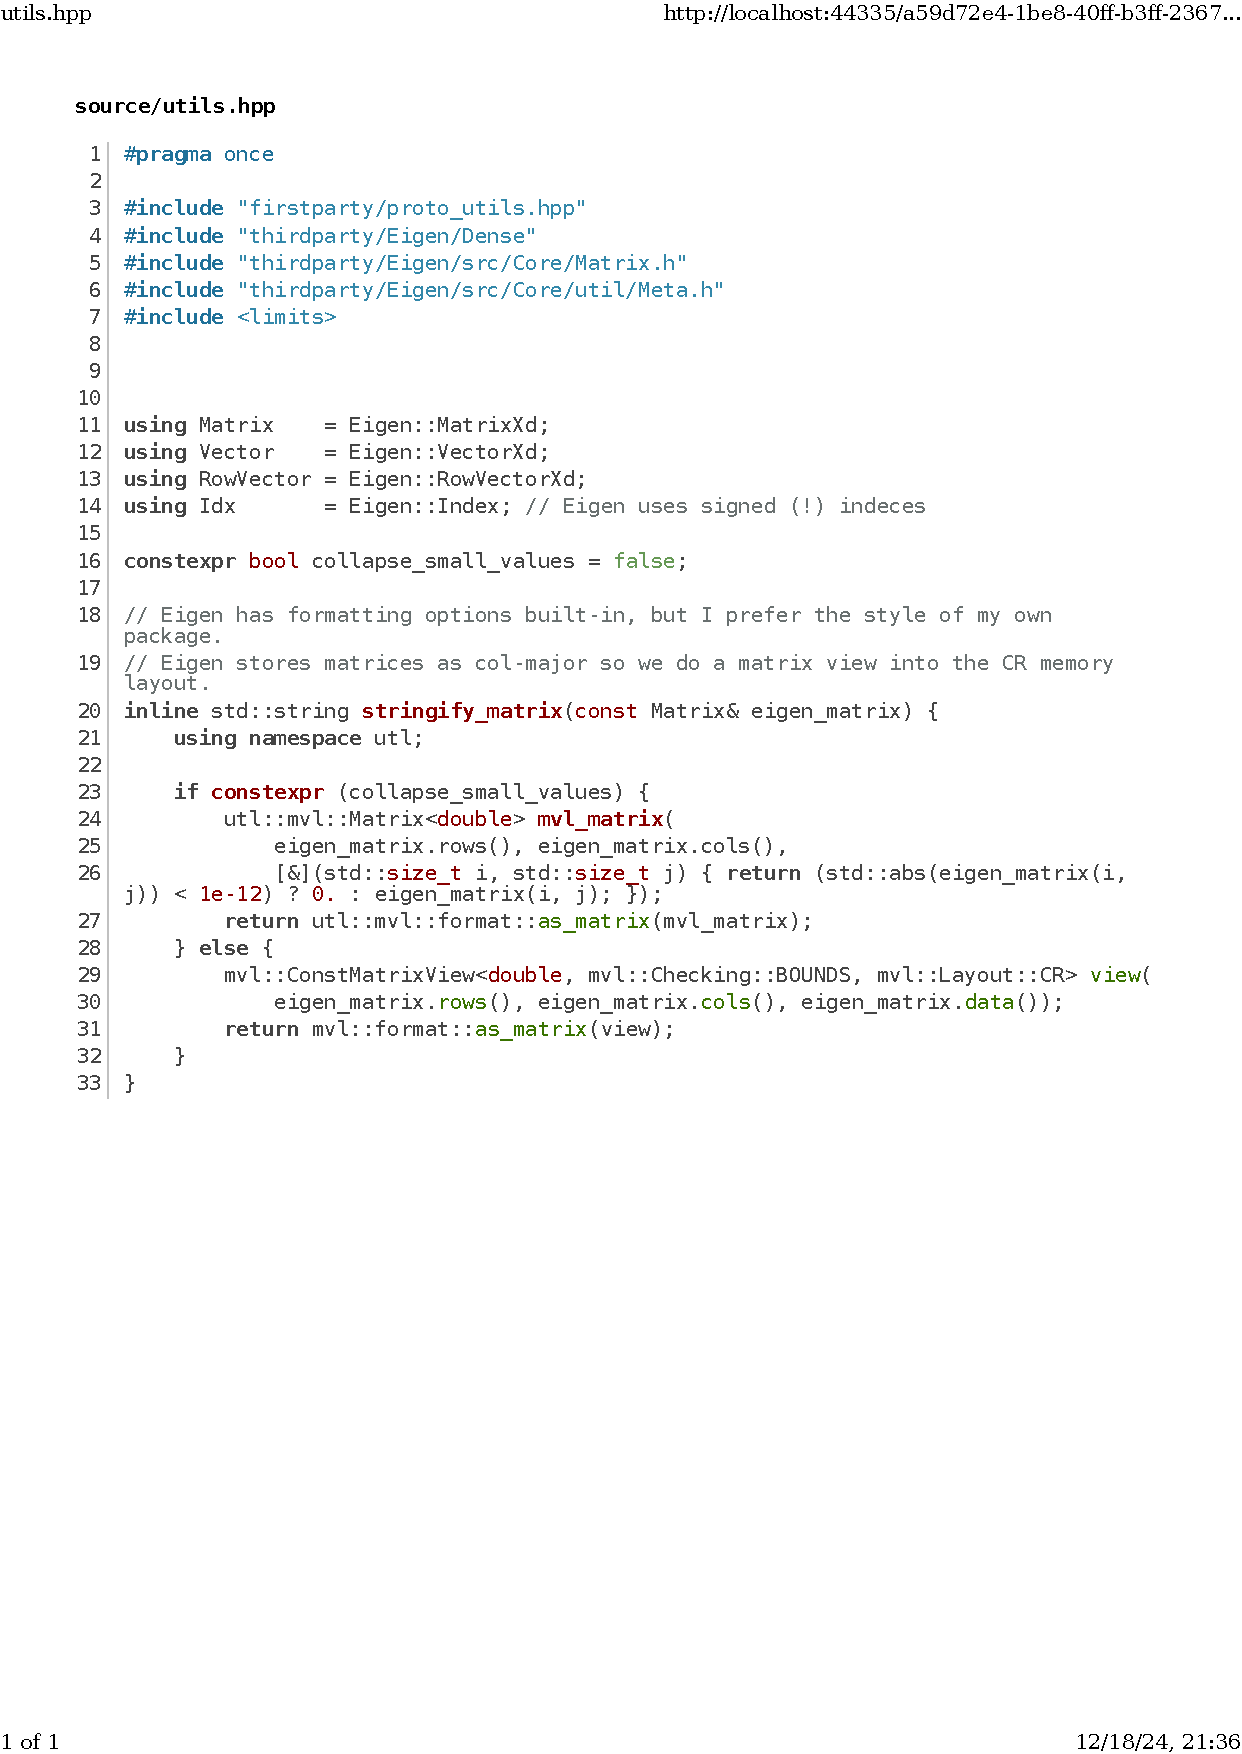
\includepdf[scale=0.9,pagecommand=\section{Листинг расчетной программы на C++}]{images/utils.hpp.pdf}
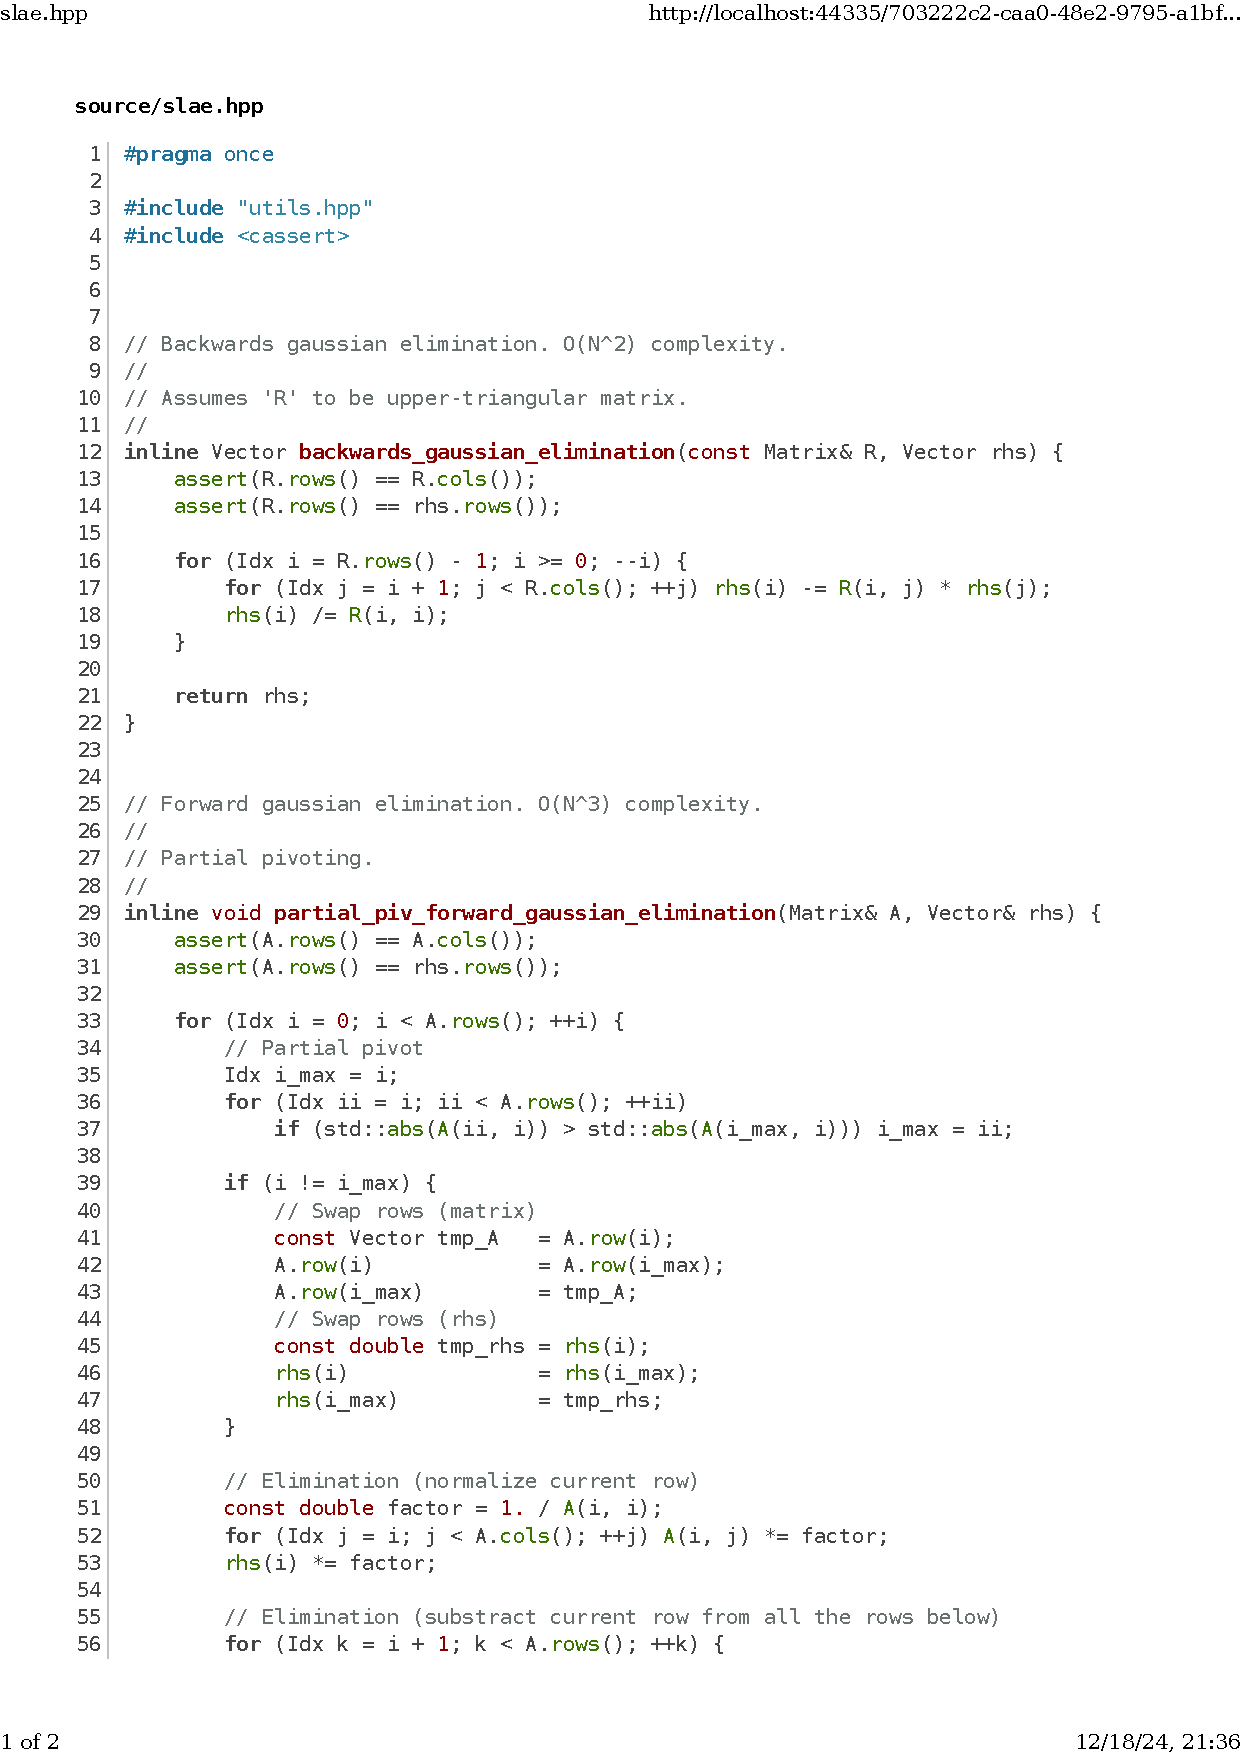
\includepdf[scale=0.9, pages=-]{images/slae.hpp.pdf}
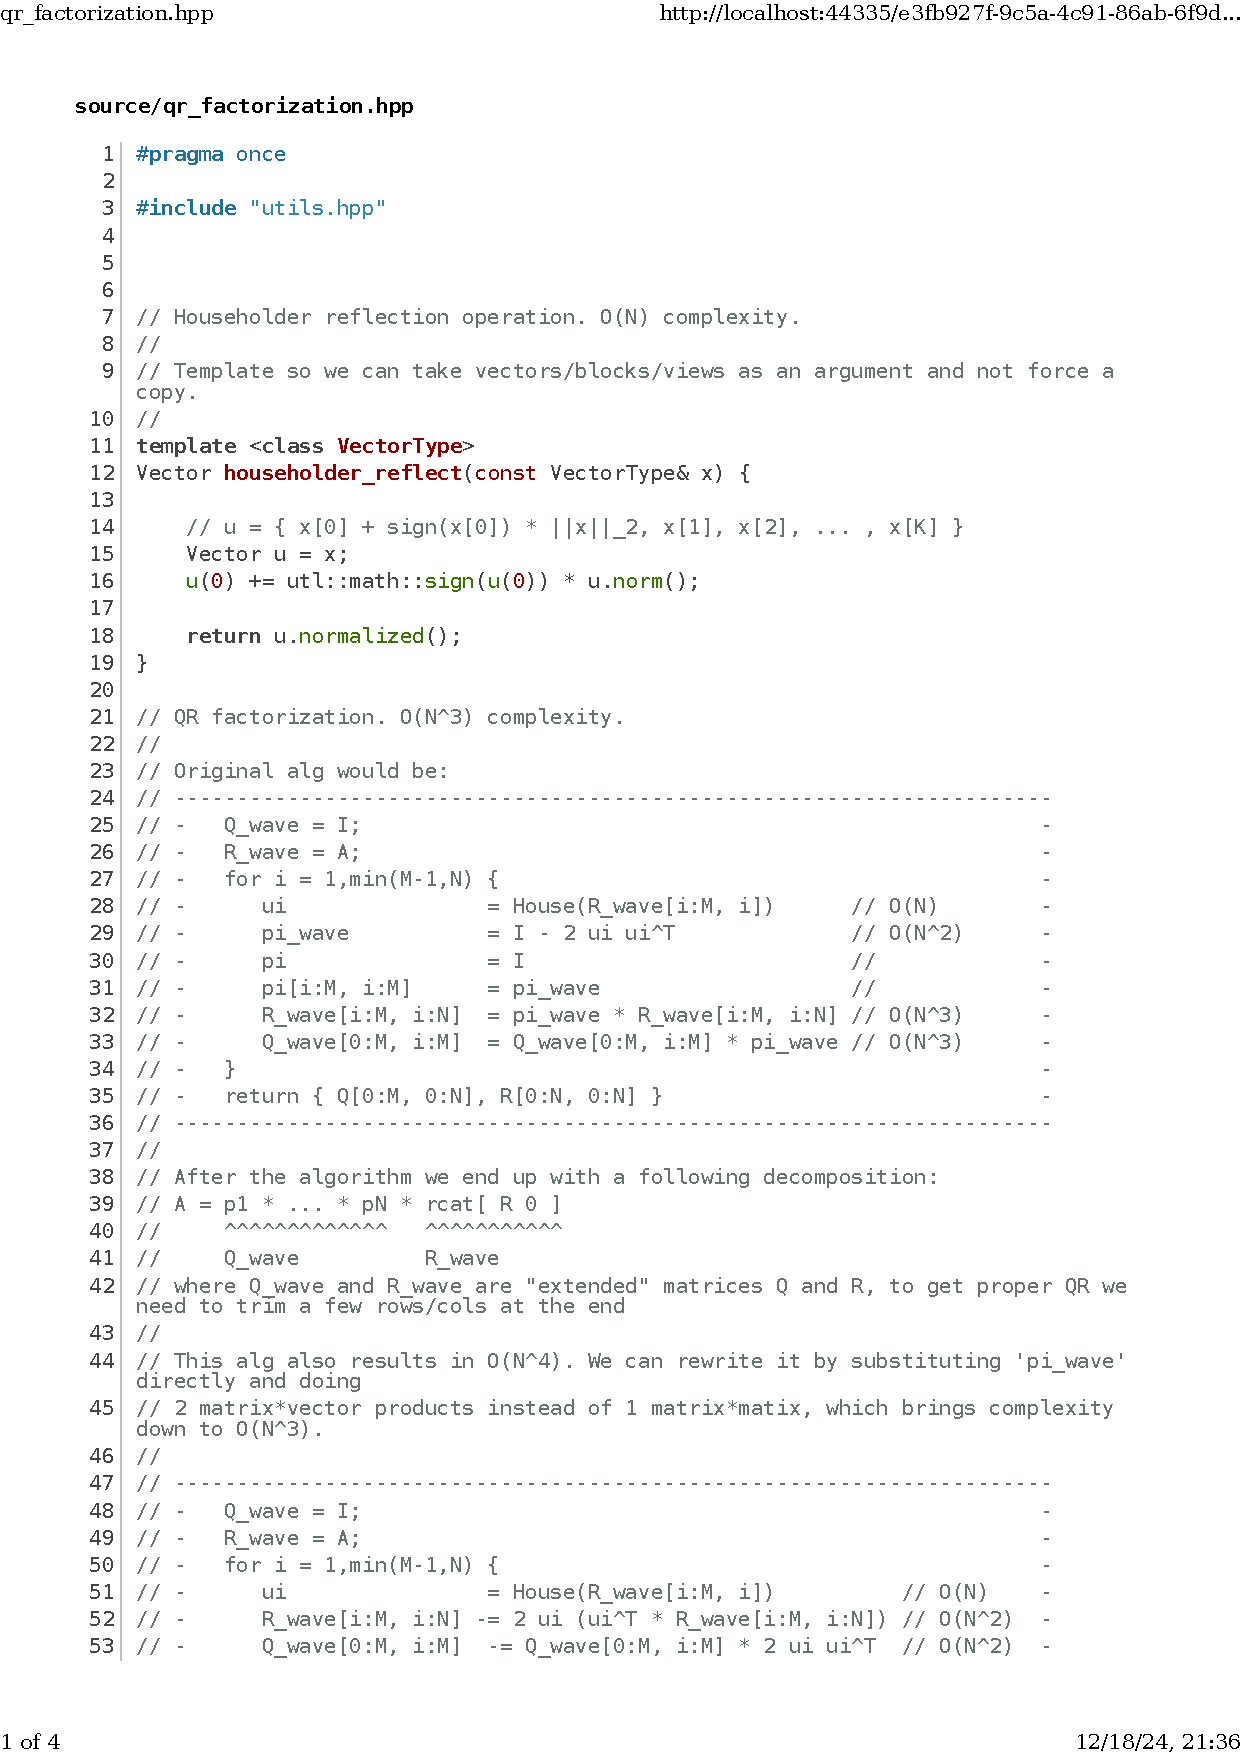
\includepdf[scale=0.9, pages=-]{images/qr_factorization.hpp.pdf}
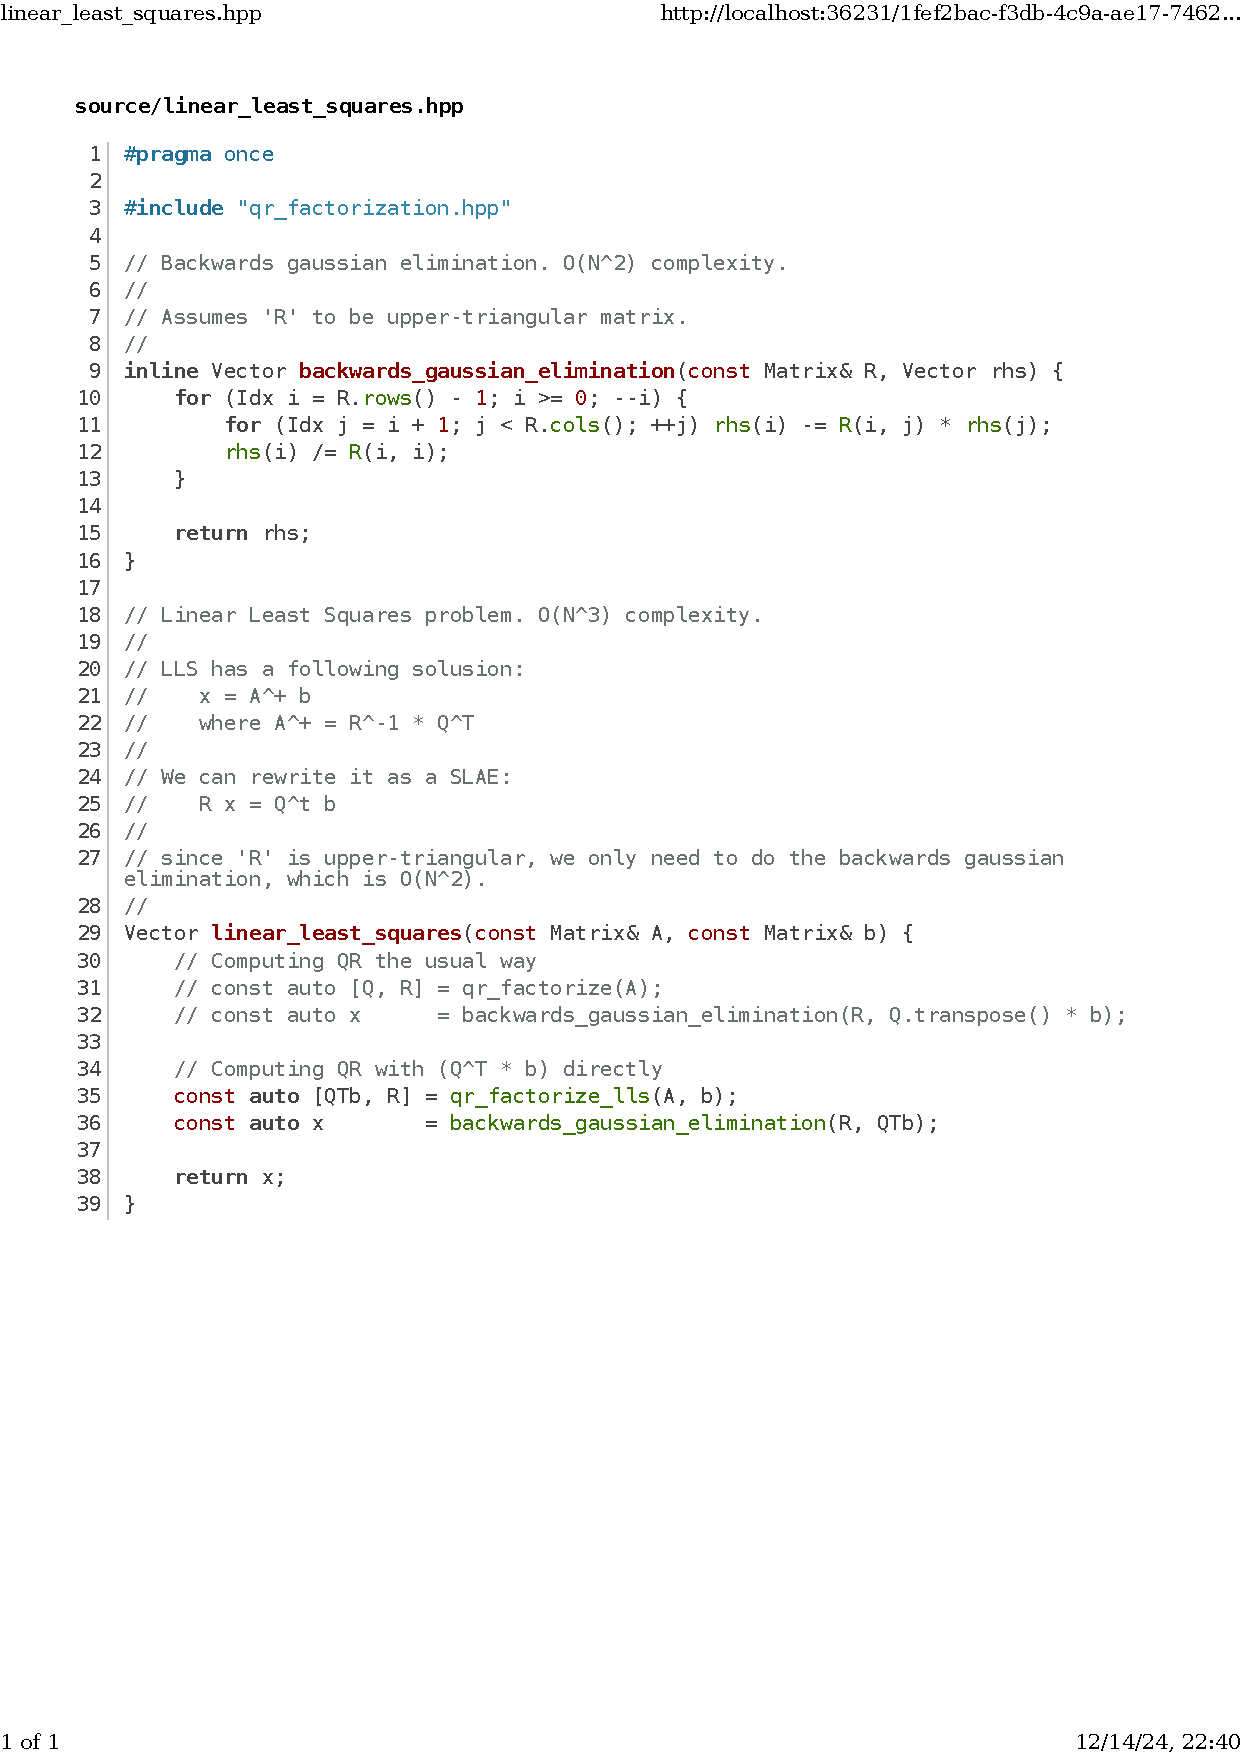
\includepdf[scale=0.9, pages=-]{images/linear_least_squares.hpp.pdf}
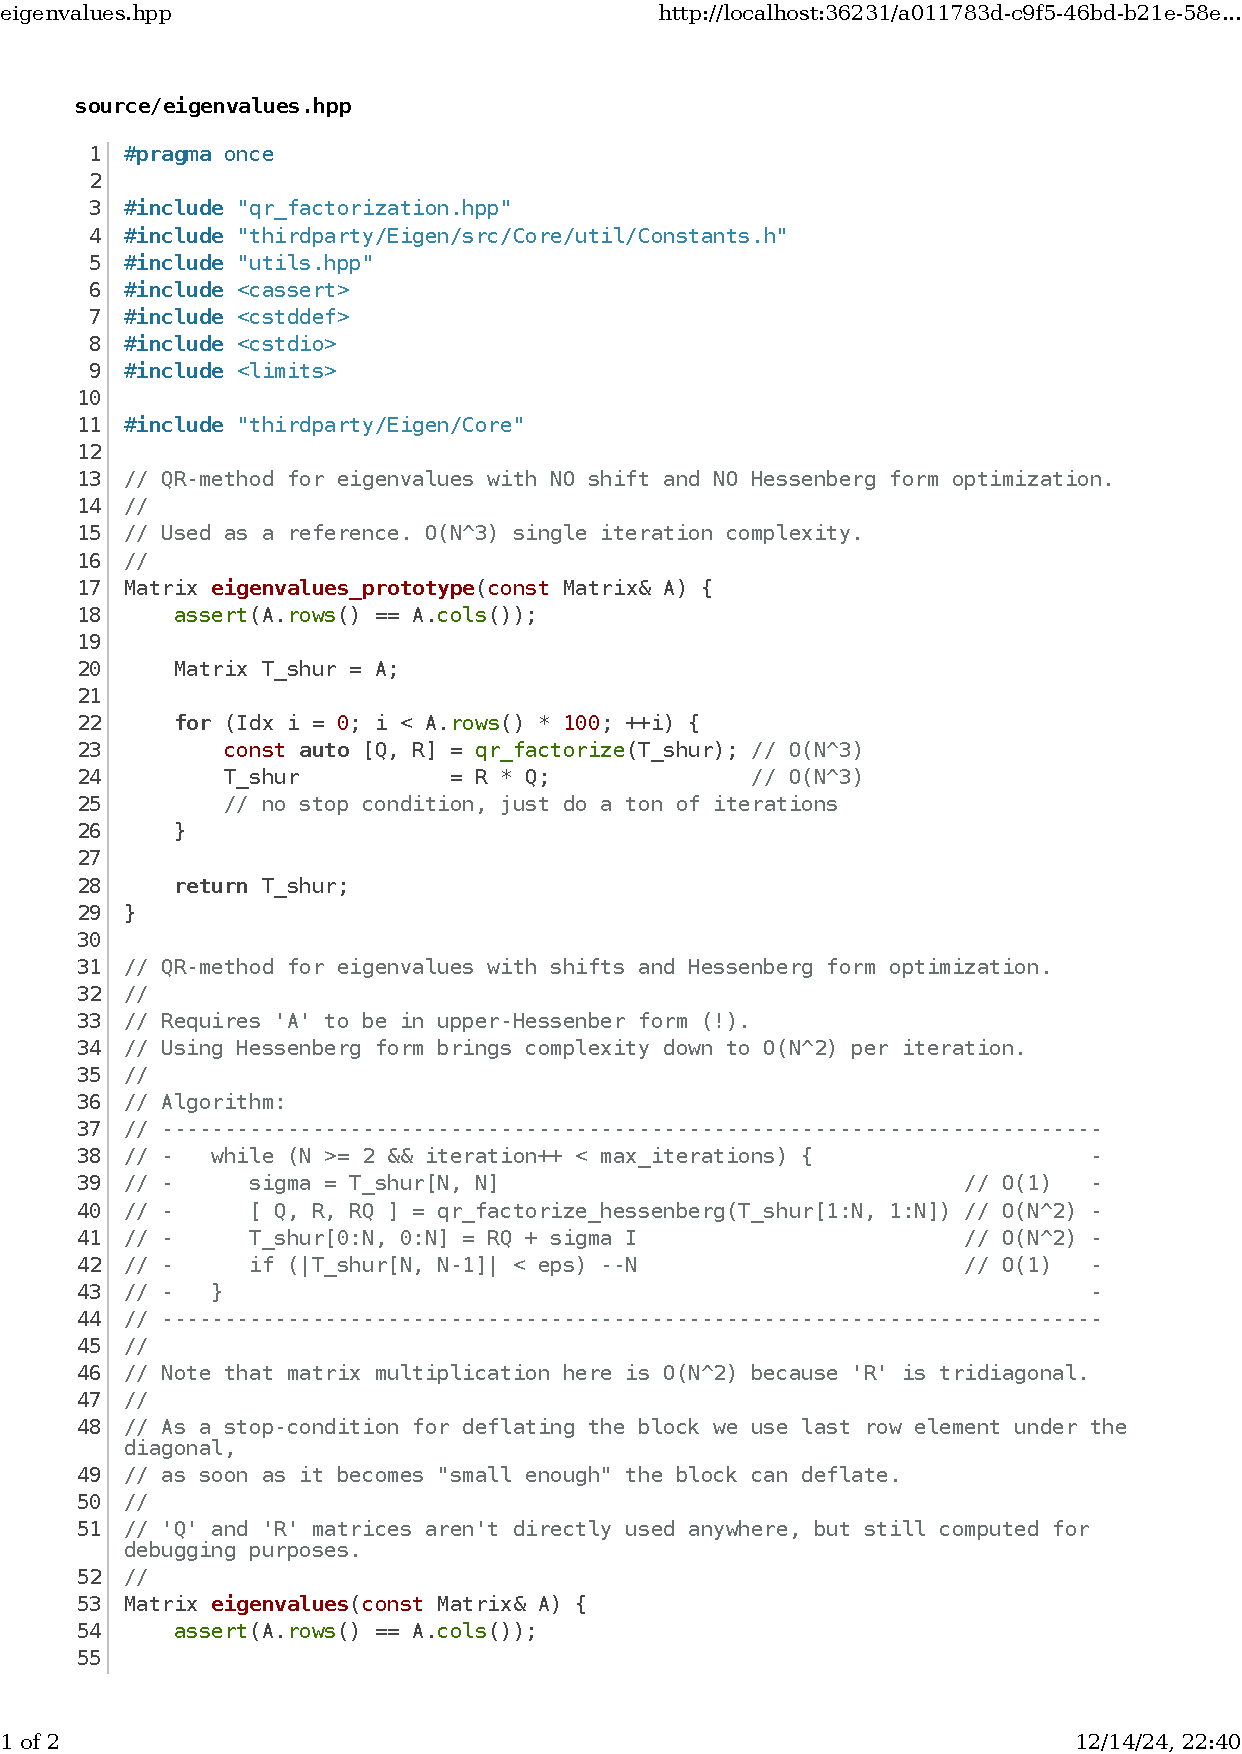
\includepdf[scale=0.9, pages=-]{images/eigenvalues.hpp.pdf}
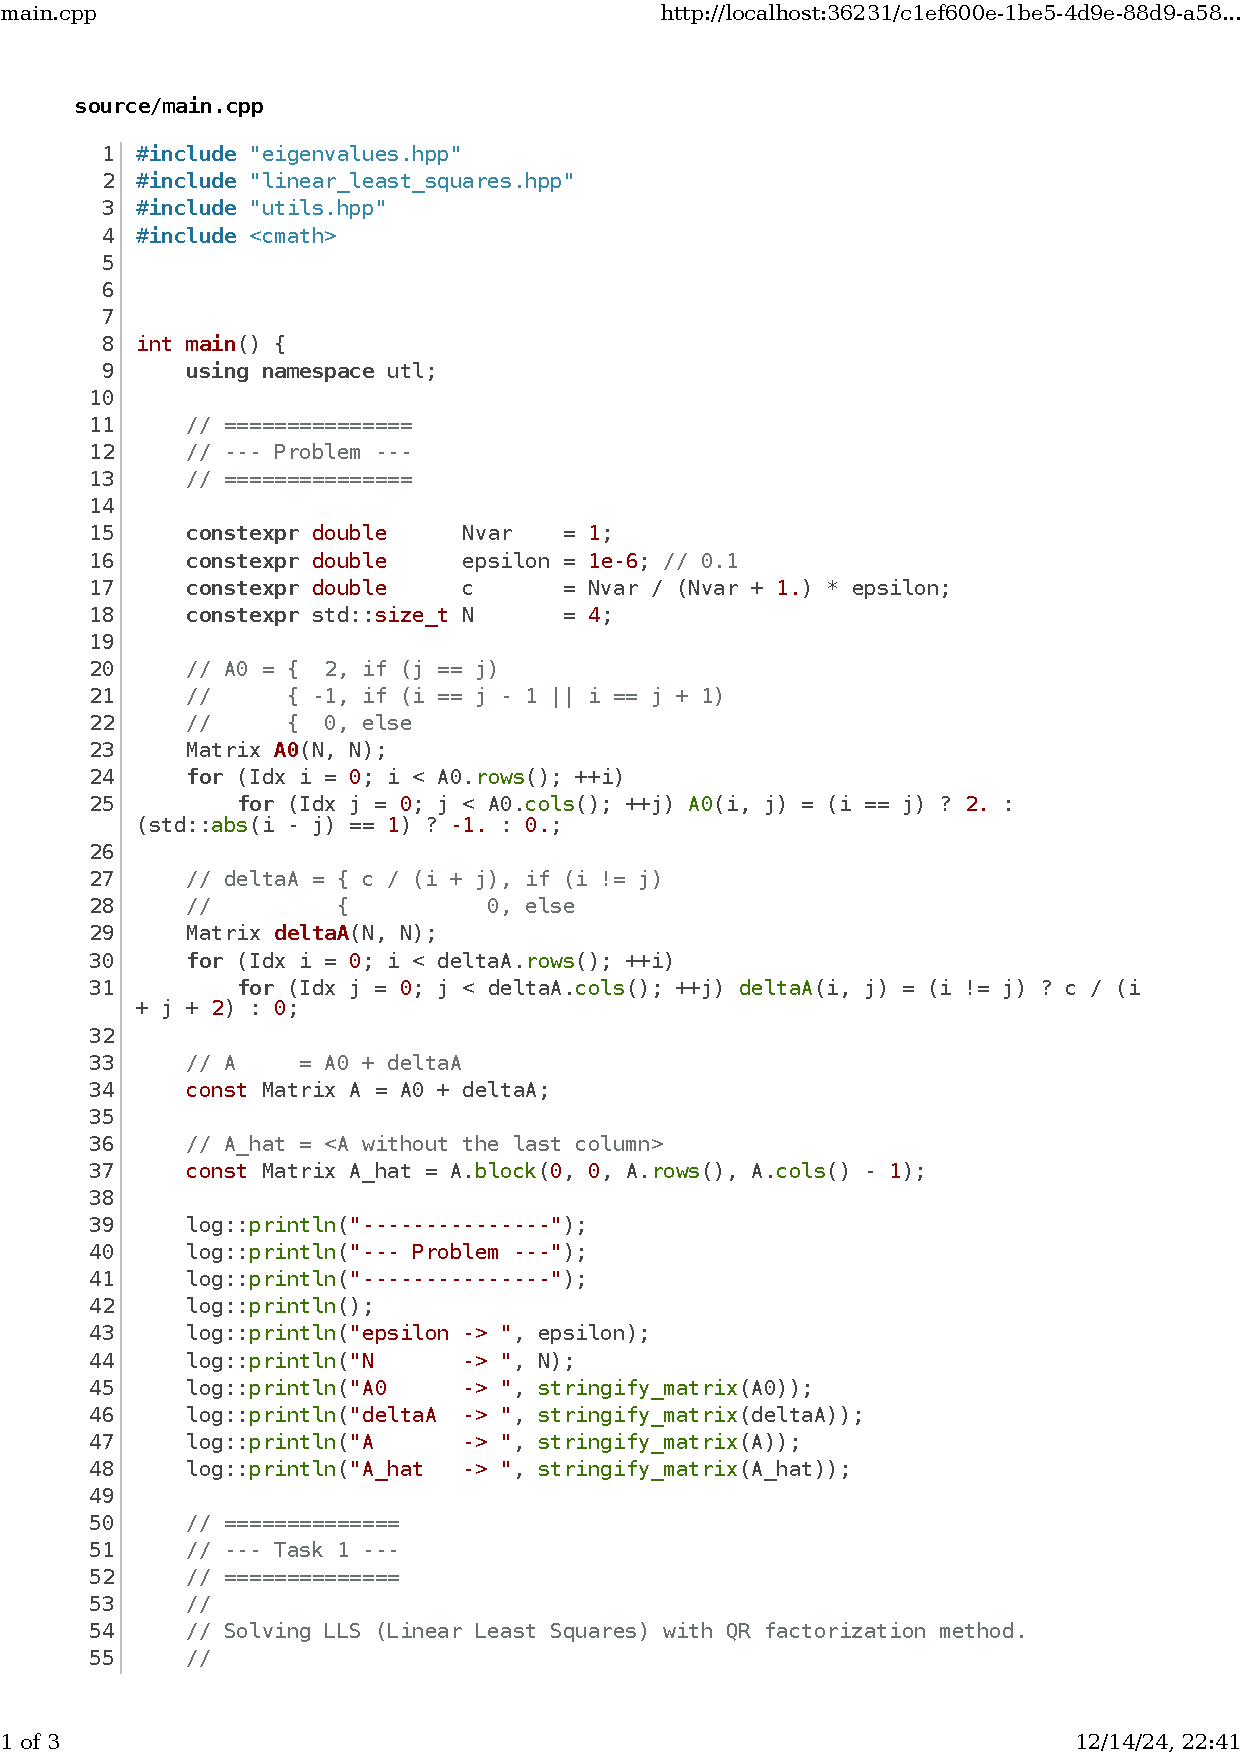
\includepdf[scale=0.9, pages=-]{images/main.cpp.pdf}

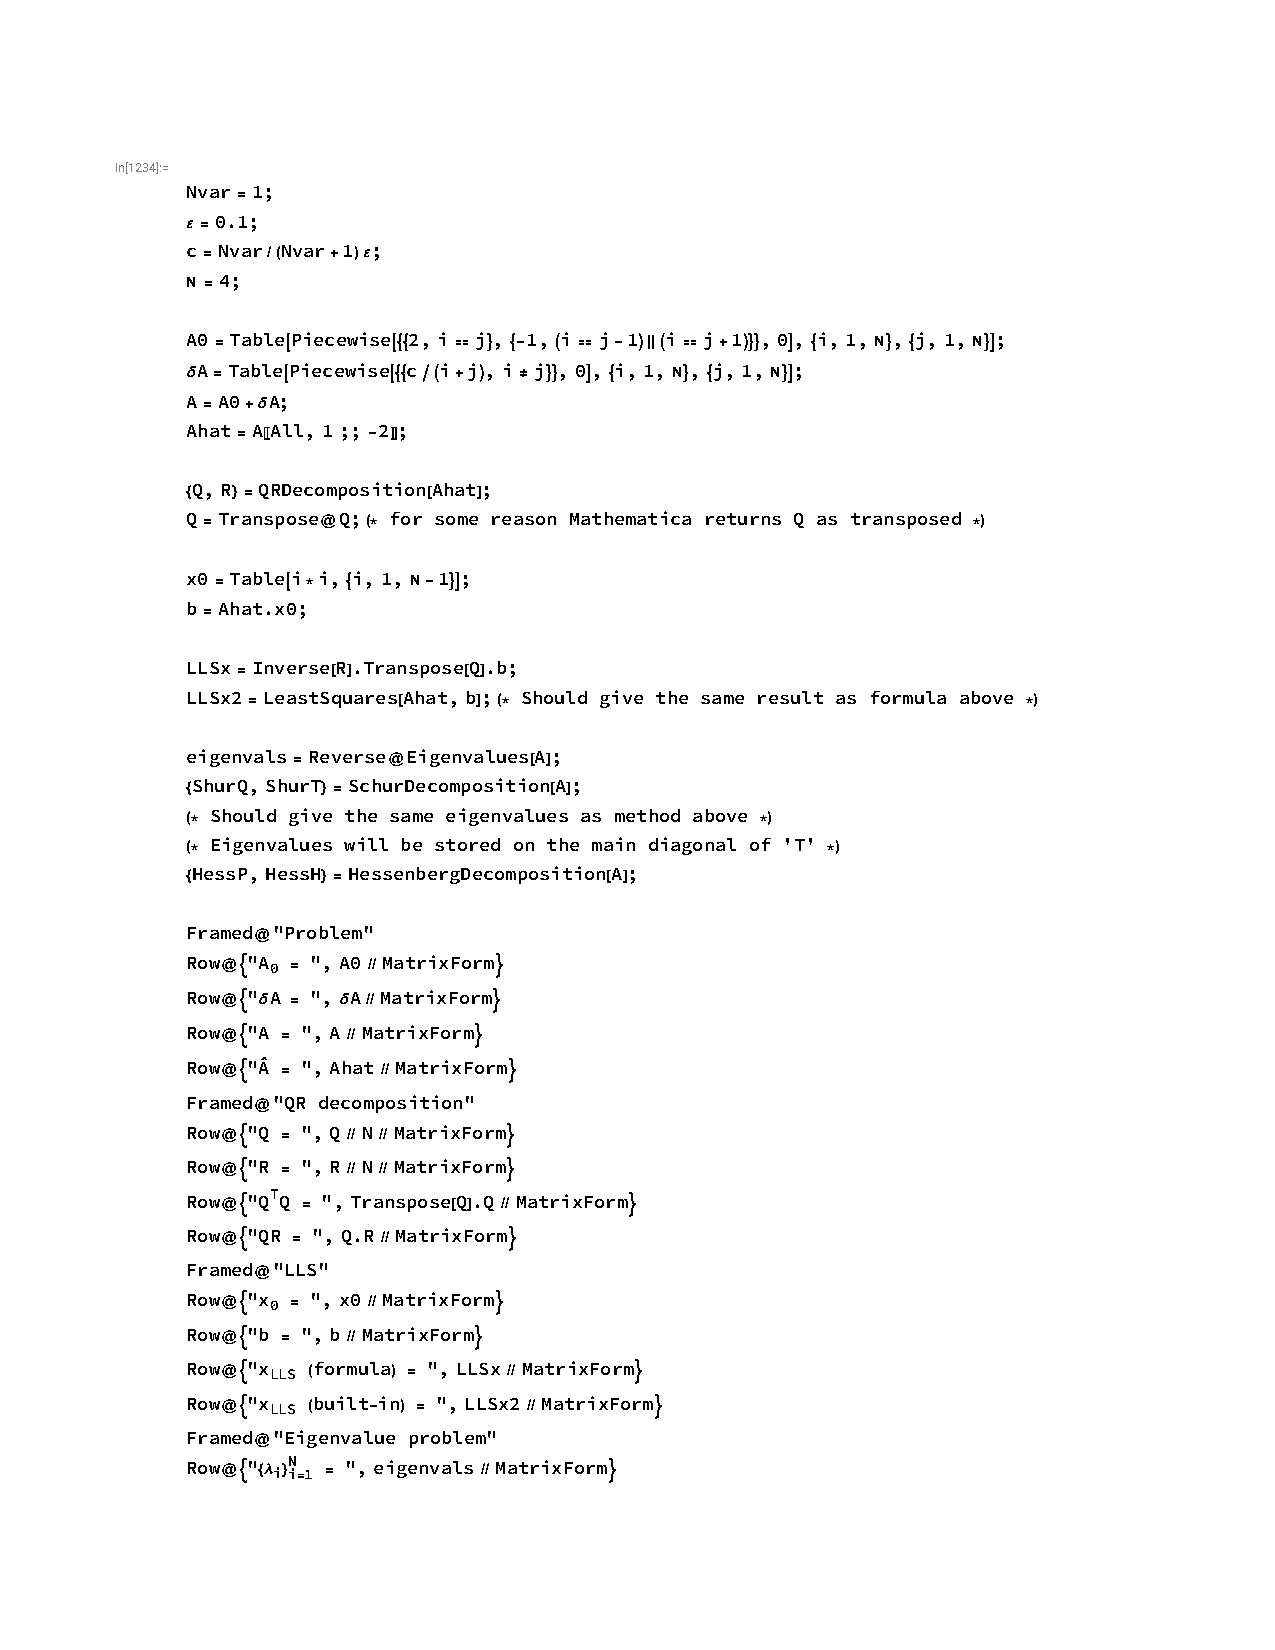
\includepdf[scale=0.9,pagecommand=\section{Листинг проверочного скрипта на Wolfram Mathematica}]{images/mathematica.pdf}

\section{Приложение. Пример сводки результатов расчетной программы}

\begin{tinyverbatim}
---------------
--- Problem ---
---------------

epsilon -> 1e-06
N       -> 4
A0      -> Dense matrix [size = 16] (4 x 4):
  [  2 -1  0  0 ]
  [ -1  2 -1  0 ]
  [  0 -1  2 -1 ]
  [  0  0 -1  2 ]

deltaA  -> Dense matrix [size = 16] (4 x 4):
  [          0 1.6667e-07   1.25e-07      1e-07 ]
  [ 1.6667e-07          0      1e-07 8.3333e-08 ]
  [   1.25e-07      1e-07          0 7.1429e-08 ]
  [      1e-07 8.3333e-08 7.1429e-08          0 ]

A       -> Dense matrix [size = 16] (4 x 4):
  [        2         -1 1.25e-07      1e-07 ]
  [       -1          2       -1 8.3333e-08 ]
  [ 1.25e-07         -1        2         -1 ]
  [    1e-07 8.3333e-08       -1          2 ]

A_hat   -> Dense matrix [size = 12] (4 x 3):
  [        2         -1 1.25e-07 ]
  [       -1          2       -1 ]
  [ 1.25e-07         -1        2 ]
  [    1e-07 8.3333e-08       -1 ]

------------------------
--- QR factorization ---
------------------------

Q             -> Dense matrix [size = 12] (4 x 3):
  [    -0.89443   -0.35857 -0.19518 ]
  [     0.44721   -0.71714 -0.39036 ]
  [ -5.5902e-08    0.59761 -0.58554 ]
  [ -4.4721e-08 -9.761e-08  0.68313 ]

R             -> Dense matrix [size = 9] (3 x 3):
  [    -2.2361      1.7889 -0.44721 ]
  [ 2.2204e-16     -1.6733   1.9124 ]
  [ -2.647e-23 -1.1102e-16  -1.4639 ]

Verification:

Q^T * Q       -> Dense matrix [size = 9] (3 x 3):
  [          1  2.7756e-16  8.3267e-17 ]
  [ 2.7756e-16           1 -2.2204e-16 ]
  [ 8.3267e-17 -2.2204e-16           1 ]

Q * R - A_hat -> Dense matrix [size = 12] (4 x 3):
  [  2.2204e-15 -1.7764e-15  6.8361e-16 ]
  [ -8.8818e-16 -8.8818e-16  1.3323e-15 ]
  [   1.327e-16  3.3307e-16 -4.4409e-16 ]
  [  3.9705e-23 -7.5843e-17  2.2204e-16 ]

-------------------------------------
--- Linear Least Squares solution ---
-------------------------------------

x0                 -> Dense matrix [size = 3] (3 x 1):
  [ 1 ]
  [ 4 ]
  [ 9 ]

b                  -> Dense matrix [size = 4] (4 x 1):
  [ -2 ]
  [ -2 ]
  [ 14 ]
  [ -9 ]

x_lls              -> Dense matrix [size = 3] (3 x 1):
  [ 1 ]
  [ 4 ]
  [ 9 ]

lls_error_estimate -> 1.8496162997539822e-16

---------------------------
--- Eigenvalue solution ---
---------------------------

H_hessenberg                  -> Dense matrix [size = 16] (4 x 4):
  [          2          1 -2.647e-23 1.3235e-23 ]
  [          1          2         -1 -2.647e-23 ]
  [  2.647e-23         -1          2          1 ]
  [ 1.3235e-23 -2.647e-23          1          2 ]

T_shur                        -> Dense matrix [size = 16] (4 x 4):
  [       3.618 -5.9746e-16 -2.7092e-16 -3.8027e-16 ]
  [  2.5614e-27     0.38197  3.9167e-16   1.396e-16 ]
  [ -2.8355e-21  1.6472e-16       2.618  -1.558e-16 ]
  [  6.2793e-18   5.744e-18 -4.3103e-23       1.382 ]

lambda0 (analythic eigenvals) -> Dense matrix [size = 4] (4 x 1):
  [ 0.38197 ]
  [   1.382 ]
  [   2.618 ]
  [   3.618 ]

lambda    (numeric eigenvals) -> Dense matrix [size = 4] (4 x 1):
  [ 0.38197 ]
  [   1.382 ]
  [   2.618 ]
  [   3.618 ]

z0      (analythic eigenvecs) -> Dense matrix [size = 16] (4 x 4):
  [ 0.37175   0.6015   0.6015  0.37175 ]
  [  0.6015  0.37175 -0.37175  -0.6015 ]
  [  0.6015 -0.37175 -0.37175   0.6015 ]
  [ 0.37175  -0.6015   0.6015 -0.37175 ]

z       (analythic eigenvecs) -> Dense matrix [size = 16] (4 x 4):
  [ 0.37175   0.6015   0.6015  0.37175 ]
  [  0.6015  0.37175 -0.37175  -0.6015 ]
  [  0.6015 -0.37175 -0.37175   0.6015 ]
  [ 0.37175  -0.6015   0.6015 -0.37175 ]

\hline
  j  &  |lambda_j^0 - lambda_j|  &  Reduction
  iterations &  ||z0_j - z-j||_2  &  Reverse iterations \\
\hline
   $1$ &                         $2.9964 \cdot 10^{-7}$ &                     $17$ &                  $7.2580 \cdot 10^{-8}$ &                   $1$ \\
   $2$ &                         $8.6690 \cdot 10^{-8}$ &                     $1$ &                  $5.3141 \cdot 10^{-8}$ &                   $1$ \\
   $3$ &                         $9.9648 \cdot 10^{-8}$ &                     $20$ &                  $6.0723 \cdot 10^{-8}$ &                   $1$ \\
   $4$ &                         $1.1331 \cdot 10^{-7}$ &                     $33$ &                  $9.0724 \cdot 10^{-8}$ &                   $1$ \\
\hline
\end{tinyverbatim}

\end{document}
